\paragraph[QuizziPedia::Front-End::Controllers\\::QuestionnaireManagementController]{QuizziPedia::Front-End::Controllers::QuestionnaireManagementController}
\begin{figure} [ht]
	\centering
	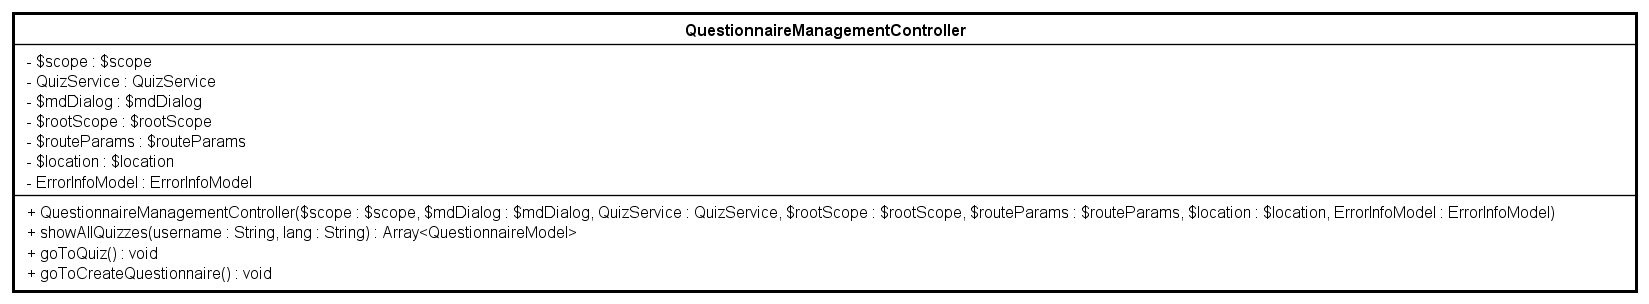
\includegraphics[scale=0.3]{UML/Classi/Front-End/QuizziPedia_Front-end_Controller_QuestionnaireManagementController.png}
	\caption{QuizziPedia::Front-End::Controllers::QuestionnaireManagementController}
\end{figure} \FloatBarrier
\begin{itemize}
	\item \textbf{Descrizione}: questa classe permette di gestire tutti i questionari creati da un utente; 
	\item \textbf{Utilizzo}: fornisce le funzionalità per recuperare dal back-end tutti i questionari creati da un utente;
	\item \textbf{Relazione con altre classi}:
	\begin{itemize}
		\item \textbf{IN \texttt{QuestionnaireManagementModelView}}: classe di tipo \textit{modelview\ped{G}} la cui istanziazione è contenuta all'interno della variabile di ambiente \$scope di \textit{Angular\ped{G}}. All'interno di essa sono presenti le variabili e i metodi necessari per il \textit{Two-Way Data-Binding\ped{G}} tra la \textit{view\ped{G}} \texttt{QuestionnaireManagementView} e il \textit{controller\ped{G}} \texttt{QuestionnaireManage-\\mentController};
		\item \textbf{IN \texttt{QuizService}}: questa classe permette di ottenere i dati di un quiz tramite delle parole chiave inserite dall'utente nella barra di ricerca;
		\item \textbf{IN \texttt{QuestionnaireModel}}: rappresenta un questionario. Contiene tutte le informazioni necessarie alla presentazione del contenuto del questionario;
	\end{itemize}
	\item \textbf{Attributi}:
	\begin{itemize}
		\item \texttt{-} \texttt{\$scope: \$scope} \\
		Campo dati contenente un riferimento all'oggetto \$scope creato da \textit{Angular\ped{G}}, viene utilizzato come mezzo di comunicazione tra il \textit{controller\ped{G}} e la \textit{view\ped{G}}. Contiene gli oggetti che definiscono il \textit{model\ped{G}} dell'applicazione;
		\item \texttt{-} \texttt{\$mdDialog: \$mdDialog} \\
		Parametro contenente un riferimento al servizio della libreria \textit{Material for Angular\ped{G}} che permette di creare delle componenti a pop-up;
		\item \texttt{-}	 \texttt{QuizService: QuizService}: permette di ottenere i dati di un quiz tramite delle parole chiave inserite dall'utente nella barra di ricerca;
		\item \rootscopeA;
		\item \routeparamsA;
		\item \locationA;
		\item \errorinfomodelA.
	\end{itemize}
	\item \textbf{Metodi}:
	\begin{itemize}
		\item \texttt{+} \texttt{QuestionnaireManagementController(\$scope: \$scope, \$mdDialog: \$mdDia-\\log, QuizService: QuizService, \$rootScope: \$rootScope, \$routeParams: \$routeParams, \$location: \$location, ErrorInfoModel: ErrorInfoModel)} \\Metodo costruttore della classe.\\
		\textbf{Parametri}: 
		\begin{itemize}
			\item \texttt{\$scope: \$scope} \\
			Campo dati contenente un riferimento all'oggetto \$scope creato da \textit{Angular\ped{G}}. Viene utilizzato come mezzo di comunicazione tra il \textit{controller\ped{G}} e la \textit{view\ped{G}}. Contiene gli oggetti che definiscono il \textit{viewmodel\ped{G}} e il \textit{model\ped{G}} dell'applicazione;
			\item \texttt{\$mdDialog: \$mdDialog} \\
			Campo dati contenente un riferimento al servizio della libreria \textit{Material for Angu-\\lar\ped{G}} che permette di creare delle componenti a pop-up;
			\item \texttt{QuizService: QuizService}: parametro che permette di ottenere, tramite il \textit{service\ped{G}}, la lista di tutte le domande presenti nel quiz;
			\item \rootscopeP;
			\item \routeparamsP;
			\item \locationP;
			\item \errorinfomodelP.
		\end{itemize}
		\item \texttt{+} \texttt{showAllQuizzes(username: String, lang: String): void} \\Metodo che ritorna tutti i questionari creati da un utente in un array di \texttt{Questionnair-\\eModel}. \\
		\textbf{Parametri}:
		\begin{itemize}
			\item \texttt{username: String}: parametro che indica l'username dell'utente del quale vogliamo scaricare tutti i questionari;
			\item \texttt{lang: String}: parametro che indica la lingua del sistema. 
		\end{itemize}
		\item \texttt{+} \texttt{goToQuiz(): void} \\Metodo che permette di andare alla pagina che gestisce le iscrizioni di un questionario;
		\item \texttt{+} \texttt{goToCreateQuestionnaire(): void} \\Metodo che permette di andare alla pagina che permette di creare un questionario.		
	\end{itemize}
\end{itemize}

